%%%%%%%%%%%%%%%%%%%%%%%%%%%%%%%%%%%%%%%%%
% Simple Sectioned Essay Template
% LaTeX Template
%
% This template has been downloaded from:
% http://www.latextemplates.com
%
% Note:
% The \lipsum[#] commands throughout this template generate dummy text
% to fill the template out. These commands should all be removed when 
% writing essay content.
%
%%%%%%%%%%%%%%%%%%%%%%%%%%%%%%%%%%%%%%%%%

%----------------------------------------------------------------------------------------
%	PACKAGES AND OTHER DOCUMENT CONFIGURATIONS
%----------------------------------------------------------------------------------------

\documentclass[12pt]{article} % Default font size is 12pt, it can be changed here

\usepackage{geometry} % Required to change the page size to A4
\geometry{a4paper} % Set the page size to be A4 as opposed to the default US Letter

\usepackage{graphicx} % Required for including pictures

\usepackage{float} % Allows putting an [H] in \begin{figure} to specify the exact location of the figure
\usepackage{wrapfig} % Allows in-line images such as the example fish picture

\usepackage{lipsum} % Used for inserting dummy 'Lorem ipsum' text into the template

\linespread{1.2} % Line spacing

%\setlength\parindent{0pt} % Uncomment to remove all indentation from paragraphs

\graphicspath{{Pictures/}} % Specifies the directory where pictures are stored

\begin{document}
	
	%----------------------------------------------------------------------------------------
	%	TITLE PAGE
	%----------------------------------------------------------------------------------------
	
	\begin{titlepage}
		
		\newcommand{\HRule}{\rule{\linewidth}{0.5mm}} % Defines a new command for the horizontal lines, change thickness here
		
		\center % Center everything on the page
		
		\textsc{\LARGE Wits University}\\[1.5cm] % Name of your university/college
		\textsc{\Large School of Electrical and Information Engineering}\\[0.5cm] % Major heading such as course name
		\textsc{\large ELEN7046 - Software Technologies and Techniques}\\[0.5cm] % Minor heading such as course title
		
		\HRule \\[0.4cm]
		{ \huge \bfseries Big Data Visualization using Commodity Hardware and Open Source Software}\\[0.4cm] % Title of your document
		
		Individual Report
		
		\HRule \\[0.6cm]
		
		
		\begin{minipage}
			{0.4
				\textwidth} 
			\begin{flushleft}
				\large \emph{Author:}\\
				Sidwell \textsc{Mokhemisa} \\
			\end{flushleft}
		\end{minipage}
		~ 
		\begin{minipage}
			{0.4
				\textwidth} 
			\begin{flushright}
				\large \emph{Student Number:} \\
				1229756 \\
				% Supervisor's Name
			\end{flushright}
		\end{minipage}
		\\[1cm]
		
		% Abstract
		\begin{flushleft}\large
			\textsc{Abstract}\\
			XXXX.
			
		\end{flushleft}
		{\large \today}\\[3cm] % Date, change the \today to a set date if you want to be precise
		
		%\includegraphics{Logo}\\[1cm] % Include a department/university logo - this will require the graphicx package
		
		\vfill % Fill the rest of the page with whitespace
		
	\end{titlepage}
	
		% Abstract
		\begin{flushleft}\large
			\textsc{Declaration of Originality}\\
			
			
		\end{flushleft}
	
	%----------------------------------------------------------------------------------------
	%	TABLE OF CONTENTS
	%----------------------------------------------------------------------------------------
	
	\tableofcontents % Include a table of contents
	
	\newpage % Begins the essay on a new page instead of on the same page as the table of contents 
	
	%----------------------------------------------------------------------------------------
	%	INTRODUCTION
	%----------------------------------------------------------------------------------------
	
	\section{Introduction} % Major section
	
XXX

\subsection{Problem Statement}

XXX

\subsection{Solution Summary}

XXX

\subsection{Approach}

%\subsubsection{Methodology}
	
		%\subsection{Executive Summary} % --optional
		
		%------------------------------------------------
		
	\section{Background}
	
	\subsection {Data Sourcing}
	
	This project was .....
	


		%--Where they come from
		%--What they currently do
		%--General experience
	
	%Example citation \cite{Figueredo:2009dg}.
	
	%------------------------------------------------
	
	%\subsection{Description of Acronyms} % Sub-section
	
	%IS - Information Systems \\
	
	%------------------------------------------------
	%Sample image for future reference (image to be taken out)
	%\begin{figure}[H] % Example image
	%\center{
\includegraphics[width=0.5\linewidth]{placeholder}}
	%\caption{Example image.}
	%\label{fig:speciation}
	%\end{figure}
	
	%------------------------------------------------
	%-------------
	%	MAJOR SECTION 1
	%----------------------------------------------------------------------------------------
	
	%\section{Problem Statement}
	
	
	
	%\subsection{Executive Summary} % --optional
	
	%------------------------------------------------
	
%	\subsection{Data Collection}
	%--Where they come from
	%--What they currently do
	%--General experience
	
	
	
	%------------------------------------------------
	
%	\subsection{Data Processing}
	


	%--Risk categories SP03
	
%	\subsubsection{Cost and Schedule}
	
	
	
	%--Earn Value Management SP01
	
	
	%--Earn Value Management SP01
	
%	\subsection{Data Visualization}
	

	%--Summary of the above
	%--Kill project/replace project manager/continue project???
	
	%------------------------------------------------
	
	\section{Lifecycle Methodology}
	
	%\subsection{Explanation Summary} %--optional
	
	%------------------------------------------------
	In order for the team to successfully deliver this project, a development methodology based on IBM Rational Unified Process (RUP) was followed albeit tailored to cater for the specific needs of this project.\\
	\\
	The diagram below depicts the IBM RUP model:
	
		\begin{figure}[H] % Example image
			\center{\includegraphics[width=1.15\linewidth]{ibm1}}
			\caption{IBM Rational Unified Process (Source: RUP, Best Practices for Software Development Teams)}
			\label{fig:speciation}
		\end{figure}
		
		
	
%	\subsection{info}
	
	
	%------------------------------------------------
	
%	\subsection{Observation} % Sub-section
	
	
%	\subsubsection{Value}
	
	
	%\\subsubsection{Risk}
	%--Risk categories SP03

%	\subsubsection{Cost \& Schedule}
	
    \section{Requirements - Use Case Models}
    
    	XXXXXX.\\
    	
    \subsection{View Elections Analytic Data}
    
    This section covers the details around the visualization Use Case. The diagram below depicts the actual Use Case followed by a table that further discusses the Use Case details:
    
    	\begin{figure}[H] % Example image
    		\center{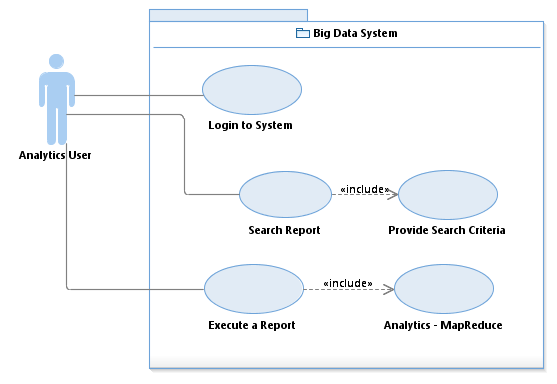
\includegraphics[width=1.15\linewidth]{UC01}}
    		\caption{Use Case Diagram - View Twitter Elections Analytics}
    		\label{fig:speciation}
    	\end{figure}
    	
  This table provides additional information to supplement the Use Case diagram.
   \begin{center}
   	\begin{tabular}{ | l | l | l | l |}
   		\hline
   		\multicolumn{1}{ |l| }{Use Case ID:} & \multicolumn{3}{| l |}{UC01}\\
   		\hline
   		\multicolumn{1}{|l|}{Use Case Name:} & \multicolumn{3}{|p{13cm}|}{View Analytics Social Media Report overlaid on map background.}\\
   		\hline
    	Created By: & Sidwell & Updated By: & Sidwell\\
    	\hline
    	Date Created: & 02/05/2016 & Date Modified: & 07/05/2016\\
    	\hline
   	\end{tabular}
   \end{center}
   \
   \
   \begin{center}
      	\begin{tabular}{ | r | p{12cm} |}
      		\hline
      	%	\multicolumn{1}{ |l| }{Use Case ID:} & \multicolumn{3}{| l |}{UC01}\\
      	%	\hline
      	%	\multicolumn{1}{|l|}{Use Case Name:} & \multicolumn{3}{|p{13cm}|}{View Analytics Social Media Report overlaid on map background.}\\
      	%	\hline
      		Actor : & Analytics User \\
      		\hline
      		Description: & This use case describes how the user will use the system to run analytics based on social media data received from Twitter.\\
      		\hline
      		Pre-conditions: & Web browser opened and user logs onto the analytics site.\\
      		\hline
      		Post-conditions: & User views requested report overlaid on map background. Drill up/ down functionality provided by the application.\\
      		\hline
      		Normal Course: & 1.	Logon to the application.
      		2.	Search report from list of available reports
      		3.	Execute a report of choice\\
      		\hline
      		Frequency of Use: & \\
      		\hline
      		Alternative Courses: & None\\
      		\hline
      		Exceptions: & None\\
      		\hline
      		Includes: & 1.	Provide search criteria or Hashtag(s).
      		2.	System runs report using Map Reduce and parallel processing in order to produce report results.\\
      		\hline
      		Special Requirements: & 1.	Ad-hoc access using most browsers (IE, Chrome, Safari).\\
      		\hline
      		Assumptions:& 1.	User login based on access to computer with browser and not necessarily integration to an LDAP compliant system.
      		2.	Support for mobile apps once developed.\\
      		\hline
      		Notes and Issues: & \\
      		\hline
      	\end{tabular}
      \end{center}
   
   
  
    	
   \subsection{Acquire Twitter Data}
	
	This section covers the details around the data acquisition Use Case. The diagram below depicts the actual Use Case followed by a table that further discusses the Use Case details:
	
		\begin{figure}[H] % Example image
			\center{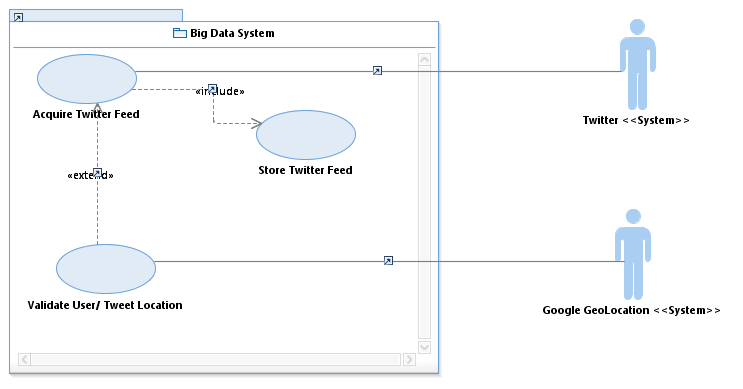
\includegraphics[width=1.15\linewidth]{UC02}}
			\caption{Use Case Diagram - Acquire Twitter Data}
			\label{fig:speciation}
		\end{figure}
		
	 This table provides additional information to supplement the Use Case diagram.
	  \begin{center}
	  	\begin{tabular}{ | l | l | l | l |}
	  		\hline
	  		\multicolumn{1}{ |l| }{Use Case ID:} & \multicolumn{3}{| l |}{UC02}\\
	  		\hline
	  		\multicolumn{1}{|l|}{Use Case Name:} & \multicolumn{3}{|p{13cm}|}{Acquire social media feed from twitter to enable big data analytics.}\\
	  		\hline
	  		Created By: & Sidwell & Updated By: & Sidwell\\
	  		\hline
	  		Date Created: & 02/05/2016 & Date Modified: & 07/05/2016\\
	  		\hline
	  	\end{tabular}
	  \end{center}
	  \
	  \
	  \begin{center}
	  	\begin{tabular}{ | r | p{12cm} |}
	  		\hline
	  		%	\multicolumn{1}{ |l| }{Use Case ID:} & \multicolumn{3}{| l |}{UC01}\\
	  		%	\hline
	  		%	\multicolumn{1}{|l|}{Use Case Name:} & \multicolumn{3}{|p{13cm}|}{View Analytics Social Media Report overlaid on map background.}\\
	  		%	\hline
	  		Actor : & Twitter and Google GeoLocation \\
	  		\hline
	  		Description: & This use case describes how data is collected from twitter based on subscribed topics stored in a database for later use in analytics processing.\\
	  		\hline
	  		Pre-conditions: & 1.	Application logs into twitter with provided credentials and starts streaming all the data that complies with subscribed topic(s).
	  		2.	Topics to subscribe to are configured on the system beforehand.
	  		3.	For each tweet streamed, the application through its orchestration service attempts to verify location from which tweet was sent, or from profile of user sending twitter using Google GeoLocation Service.
	  		4.	Where location could not be verified, the tweet is stored in the database without location information.
	  		\\
	  		\hline
	  		Post-conditions: & 1.	Developed application authenticates and streams data.
	  		2.	Streamed data is stored in the database with location information where location could be determined.\\
	  		\hline
	  		Normal Course: & 1.	Configure election related topics to subscribe to (both US and SA).
	  		2.	Allow application to log onto both twitter and Google GeoLocation.
	  		3.	Stream tweets through orchestration service while attempting to verify location by validating certain data via Google GeoLocation Service.
	  		4.	Store all tweets regardless of location information availability.\\
	  		\hline
	  		Frequency of Use: & \\
	  		\hline
	  		Alternative Courses: & None\\
	  		\hline
	  		Exceptions: & None\\
	  		\hline
	  		Includes: & 1.	Storing of tweeter feeds in a database.\\
	  		\hline
	  		Special Requirements: & 1.	Username token provided by twitter.
	  		2.	Username token provided by Google GeoLocation Service.
	  		3.	Internet access to connect to both services.\\
	  		\hline
	  		Assumptions:& 1.	Availability of infrastructure resources to harvest more than a million twitter records and store them.\\
	  		\hline
	  		Notes and Issues: & \\
	  		\hline
	  	\end{tabular}
	  \end{center}
	  
	 

	\section{Assumptions and Constraints}
	
	Early  
	%------------------------------------------------
	\section {Design Decisions}
	
	The table below details all the key design decisions made in the delivery of the solution:
	
\begin{itemize} 
	\item \textbf{History Data:} History data/ batch....
\end{itemize}
	
	
	
	%\subsection{Explanation Summary} %--optional

	%------------------------------------------------
	
	%--Earn Value Management 
	
	
	%--Summary of the above
	%--Kill project/replace project manager/continue project???

	
	\section{Solution Design}
		
	\subsection{High Level Design: Component Architecture}
	The high level component model below depicts the key features of the solution delivered for the project.
	
	
		\begin{figure}[H] % Example image
			\center{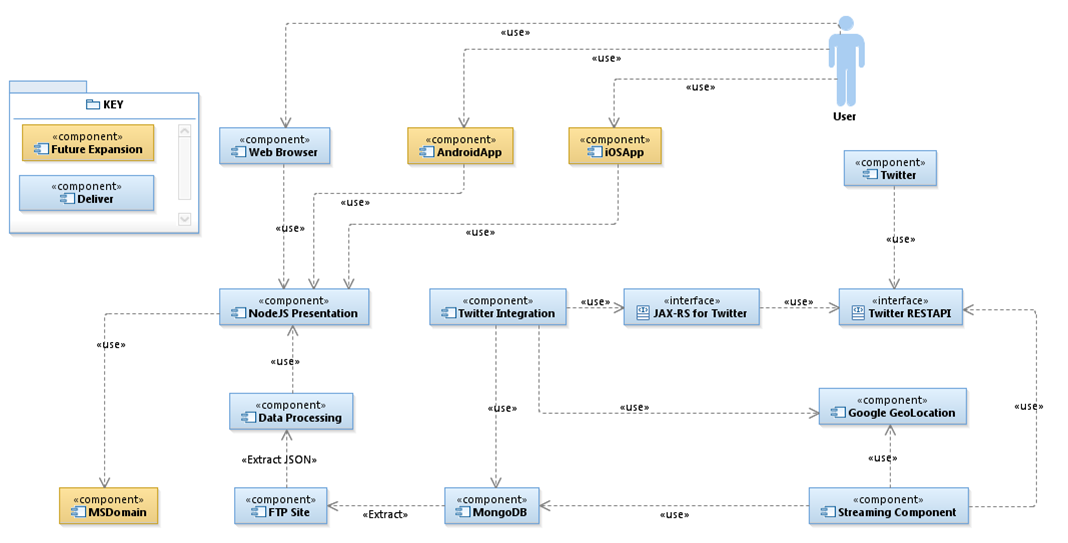
\includegraphics[width=1.15\linewidth]{HLD1}}
			\caption{High Level Component Model.}
			\label{fig:speciation}
		\end{figure}
		
		
	\subsection{Solution Sequence Diagrams}
	
		\begin{figure}[H] % Example image
			\center{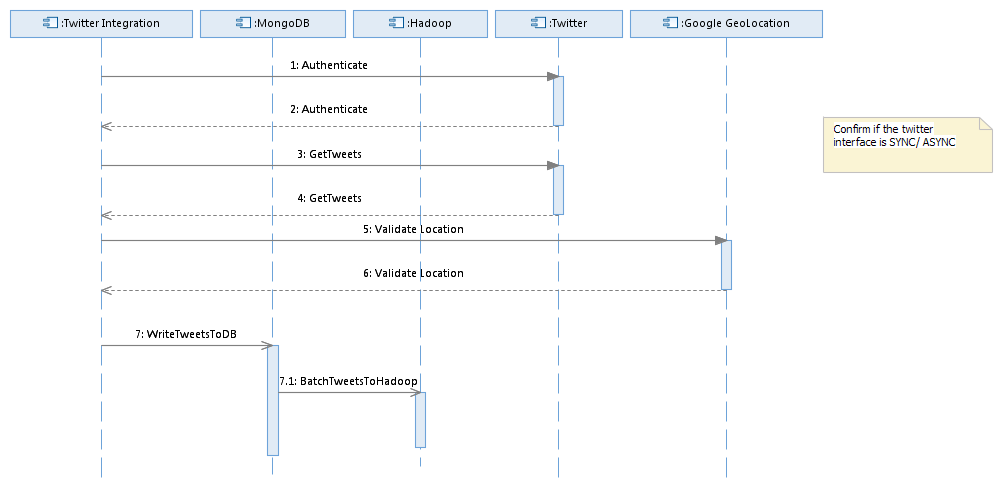
\includegraphics[width=1.15\linewidth]{SD_JEE}}
			\caption{Sequence Diagram: Data Integration - History}
			\label{fig:speciation}
		\end{figure}
	

	\subsection{Operational Model: Infrastructure Design}
	
	The Raspberry Pi 
	
		\begin{figure}[H] % Example image
		\center{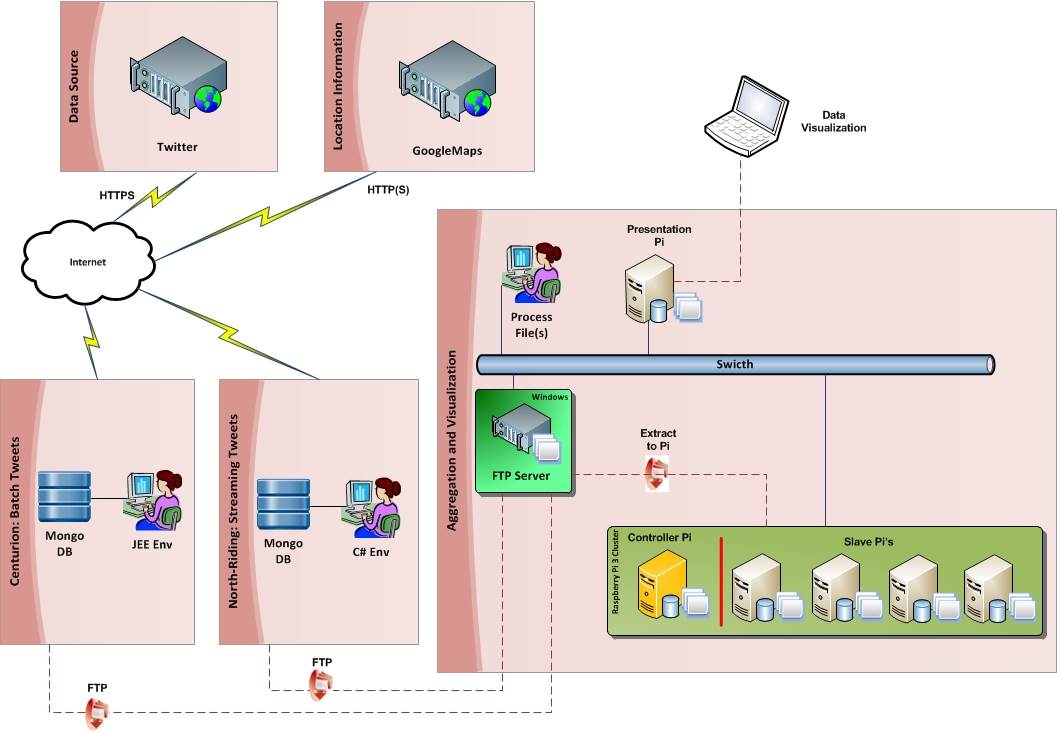
\includegraphics[width=1.15\linewidth]{OM1}}
			\caption{Operational Model: Phyical}
			\label{fig:speciation}
		\end{figure}
	
	

	
	The project 
	
	%	CONCLUSION
	%----------------------------------------------------------------------------------------
	
	\section{Conclusion} % Major section
	
	All this hardware and software is available to anybody interested in Big Data processing.\\
	
	The hardware is cheap and the software is free.\
	
	The learning curve in the beginning can be quite steep but is ultimately very rewarding in terms of what can be achieved with so little financial investment.
	
	
	
	
	\newpage
	
	%----------------------------------------------------------------------------------------
	%	BIBLIOGRAPHY
	%----------------------------------------------------------------------------------------
	
	\begin{thebibliography}{99} % Bibliography - this is intentionally simple in this template
		
		\bibitem 1. S. Madam. From Databases to Big Data. IEEE Computer Society, 2012.
	
		%\newblock 
		
		\bibitem 2. V. Kumar, R. Yuvaraj, C. Anusha. Effective Distribution of Large Scale Datasets Clustering Based on MapReduce. 2016.

		
	\end{thebibliography}
	
	\section{Appendices}
	
	%----------------------------------------------------------------------------------------
	
\end{document}